\documentclass[12pt]{article}
\usepackage[margin=3cm]{geometry}
\usepackage[portuguese]{babel}
\usepackage[utf8]{inputenc}
\usepackage{fancyhdr}
\usepackage{hyperref}
\usepackage{indentfirst}
\usepackage[pdftex]{graphicx}
\usepackage{siunitx}

\urlstyle{same}
\pagestyle{fancy}
\fancyhf{}
\author{
	Grupo: al024\\Alunos: António Coelho (ist195535) e Gustavo Aguiar (ist195587)
}
\title{Relatório 1º Projeto ASA 2020/2021}
\date{}
\hypersetup{
    colorlinks=true,
    linkcolor=black,
    filecolor=black,      
    urlcolor=cyan,
}
\fancyfoot[C]{\thepage}
\begin{document}
\maketitle
\section{Descrição do Problema e da Solução}
O problema foi interpretado como um de grafos (em específico um \emph{DAG}), em que as peças de dominós correspondem a vértices e as dependências entre os mesmos a arcos. Concluiu-se que o número de intervenções necessárias para garantir que todas as peças caiam é dado pelo menor número de vértices a partir dos quais se pode percorrer todo o grafo, i.e., a quantidade de fontes\footnote{Uma fonte é um vértice com grau de entrada zero.} no DAG. Do mesmo modo, determinou-se que o tamanho da maior sequência de peças a caírem representa o número de vértices no caminho mais longo do \emph{DAG}.
Assim, como auxílio de resolução dos problemas encontrados utilizaram-se as seguintes referências:
\begin{itemize}
\item\href{https://www.geeksforgeeks.org/topological-sorting-indegree-based-solution/}{Algoritmo de Kahn para ordenação topológica}
\item\href{https://www.mathcs.emory.edu/~cheung/Courses/171/Syllabus/11-Graph/Docs/longest-path-in-dag.pdf}{Artigo de Mumit Khan, CSE 211: Descobrir o caminho mais longo num \emph{DAG}}
\end{itemize}
 
 \section{Análise Teórica}
A representação do \emph{DAG} em memória foi feita com recurso a uma lista de adjacências - complexidade de espaço $\Theta{(V+E)}$ - assumindo que o grafo não apresentava uma densidade elevada, fruto da natureza real do problema. Assim, dada a representação em lista de adjacências e com vista ao desempenho, procurou-se dar uso a algoritmos que corressem em tempo linear de acordo com o tamanho do grafo\footnote{Tamanho do grafo é dado por \href{https://bit.ly/3gfDEJJ}{$\left|V\right|+\left|E\right|$}.} - $O(V+E)$.

A solução visada para a resolução dos problemas apresentados consiste em 3 etapas: ler o \emph{DAG} de \emph{input} (\underline{1}), ordenar topologicamente o \emph{DAG} (\underline{2}) e para cada vértice em ordem topologicamente linear percorrer a sua lista de adjacências a fim de encontrar o maior caminho no \emph{DAG} (\underline{3}).

Para (\underline{1}) - leitura de \emph{input} - usando \texttt{scanf}, ler os dados de entrada dentro de um ciclo a depender linearmente de E, i.e., $O(E)$.

Para (\underline{2}) - ordenar topologicamente o \emph{DAG} - percorrer os vértices do \emph{DAG} adicionando a uma \emph{stack} os de grau de entrada zero. Para cada um desses adicioná-lo à ordenação topológica e visitar os seus adjacentes; decrementar em 1 valor o grau de entrada dos adjacentes (remover o arco do \emph{DAG}) e adicioná-los à \emph{stack} se ficarem com grau de entrada 0. Repetir o processo para cada vértice na stack. Logo, $O(V+E)$.

Para (\underline{3}) - encontrar o maior caminho do \emph{DAG} - para cada vértice $v$ $\in{V}$ em ordenação linear calcular dist($v$)=$max_{(u,v)\in{E}}$\{dist($u$)+1\} e devolver $max_{(v)\in{V}}$\{dist($v$)\}, onde dist($v$) representa a maior distância entre uma fonte do \emph{DAG} ao vértice $v$. Logo, $O(V+E)+O(V+E) = O(2V+2E) = O(V+E)$.

Conclui-se que a complexidade geral da solução aos problemas é dada por $O(E)+O(V+E)+O(V+E) = O(2V+3E) = \textbf{O(V+E)}$.

\section{Avaliação Experimental dos Resultados}
Para a devida análise do algoritmo implementado, utilizou-se um computador com processador \emph{Intel Core i5 Quad-Core} a \SI{1,4}{GHz}, com \SI{8}{GB} de memória RAM, com o sistema operativo \emph{macOS Big Sur}.

Utilizou-se a ferramenta \texttt{randomDAG} fornecida pelo corpo docente da unidade curricular de ASA para gerar \emph{DAGs} de tamanho variável até à ordem de grandeza de $10^6$, com probabilidade de densidade de arco $p=0.4$, bem como a chamada de sistema \texttt{time} com o intuito de cronometrar o desempenho do algoritmo implementado dado \emph{DAGs} de \emph{input} gerados pelo \texttt{randomDAG}.

\begin{center}
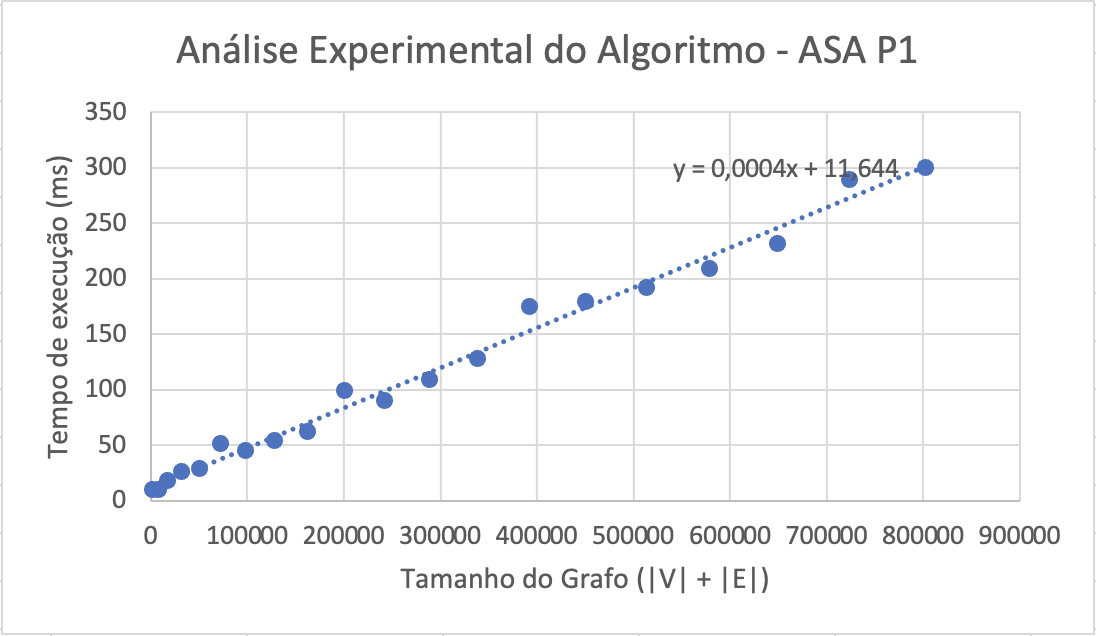
\includegraphics[width=\linewidth]{reglinear.png}
\end{center}	

Por fim, utilizou-se a ferramenta \emph{Microsoft Excel}, registando-se os valores obtidos da testagem e  ajustou-se uma regressão linear que demonstra, experimentalmente, a veracidade da complexidade do algoritmo esperada teoricamente, vendo que o tempo de execução tem uma relação linear com o tamanho do grafo - $\textbf{O(V+E)}$.


\end{document}